\part{Hardware}
\section{Komponenten}
Die \ref{fig:UebHardware} zeigt das Zusammenspiel der unterschieldichen Komponetne vereinfacht dargestellt. Die Hauptkomponenten bilden dabei die Energieversorgung, der Antrieb zur Erzuegung der Drehbewegung, das Embedded Sytsem zur Erfassung der Geschwindigkeit und der PC zur Programmierung und Auswertung der generierten Daten.
\begin{figure}[ht]
    \centering
    %    \missingfigure{Bild einfügen}
    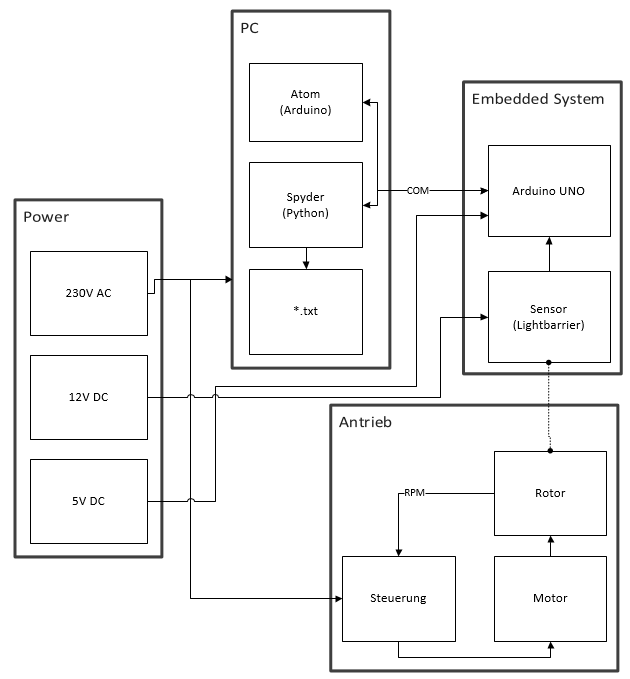
\includegraphics[width=\textwidth]{images/UebersichtVisio}
    \caption{Übersicht der Hardware}
    \label{fig:UebHardware}
\end{figure}
\subsection{Technische Daten der Lichtschranke}
\null\marg{Lichtschranke}
\begin{tabular}{ll}
    Hersteller & Panasonic\\
    Typ & Einweglichtschranke\\
    Modellnummer &  EX-21A-PN \\
    Schalttyp & Hell-EIN\\
    Reichweite & 1m\\
    Wiederholpräzision & max. 0.05 mm\\
    Ansprechzeit & max. 0.5 ms\\
    Spannung & 12 bis 24V DC $\pm$ 10\% \\
    Stromaufnahme & max. 10 mA
\end{tabular}
\\\null\\

Die kompletten Technischen Daten findet man in Anhang \ref{app:ex20}.\\

Bei der Auswahl der Lichtschranke wurde vor allem drauf geachtet, dass sie eine schnelle Reaktionszeit hat sowie eine gute Wiederholpräzision Weiter war es wichtig, dass sie Aktiv-Low ist, da nicht alle Arduinos auf ein HIGH-Signal einen Interrupt auslösen können.\\
\clearpage

\subsection{Arduino}
Als \marg{Arduino Uno} Embedded System wird ein Arduino Uno verwendet. Er wird wie in \ref{fig:ArdAns} gezeigt angeschlossen. Um die Ausgangsspannung der Lichtschranke von 12V auf das 5V-Level des Arduinos zu reduzieren wird ein Spannungsteiler verwendet. Die Berechnung dazu findet sich im Anhang \ref{app:berechnung}.\\


Für den Anschluss\marg{Anschluss} der Peripherie werden folgende Pins benötigt:\newline
\begin{tabular}{ll}
    \textbf{Pin} & \textbf{Bezeichnung}\\
    2 & Lichtschranke 1 (LB1)\\
    3 & Lichtschranke 2 (LB2)\\
\end{tabular}

\begin{figure}[ht]
    \centering
%    \missingfigure{Bild einfügen}
    \begin{subfigure}[c]{0.8\textwidth}       
        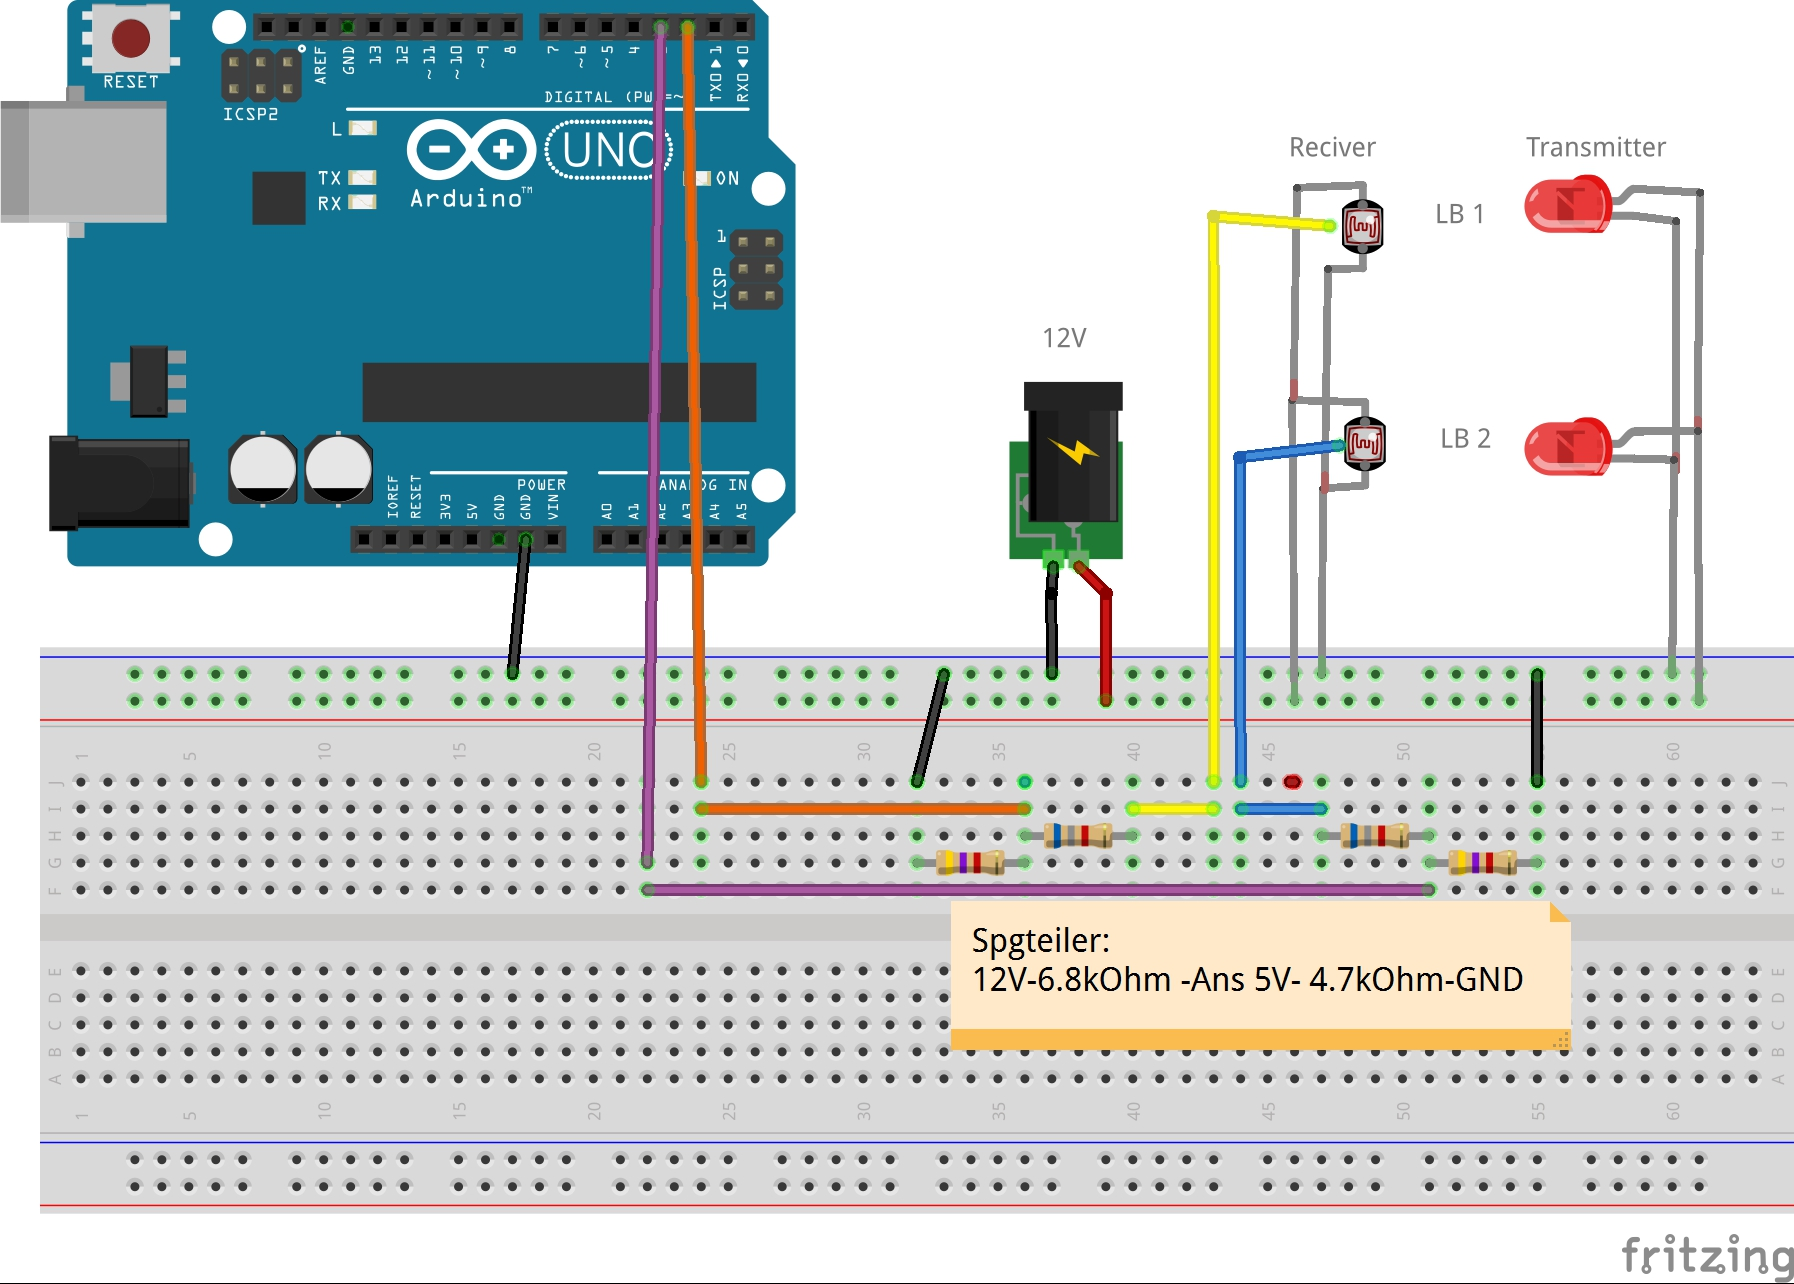
\includegraphics[width=\textwidth]{images/fritzing.jpg}
%        \subcaption{Übersicht}   
\null       
    \end{subfigure}
    
    \begin{subfigure}[c]{0.8\textwidth}
        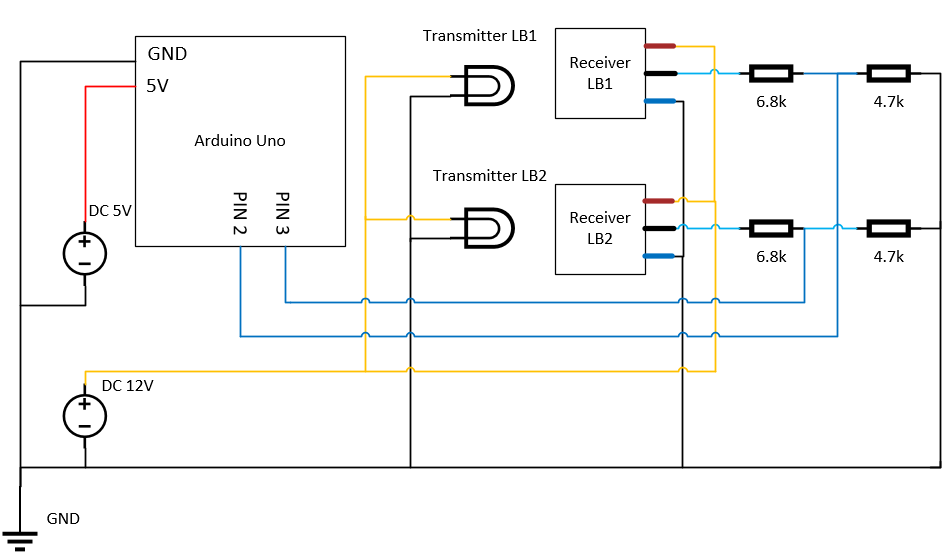
\includegraphics[width=\textwidth]{images/SchemaVisio.png}
%        \subcaption{Detail}
    \end{subfigure}
%   	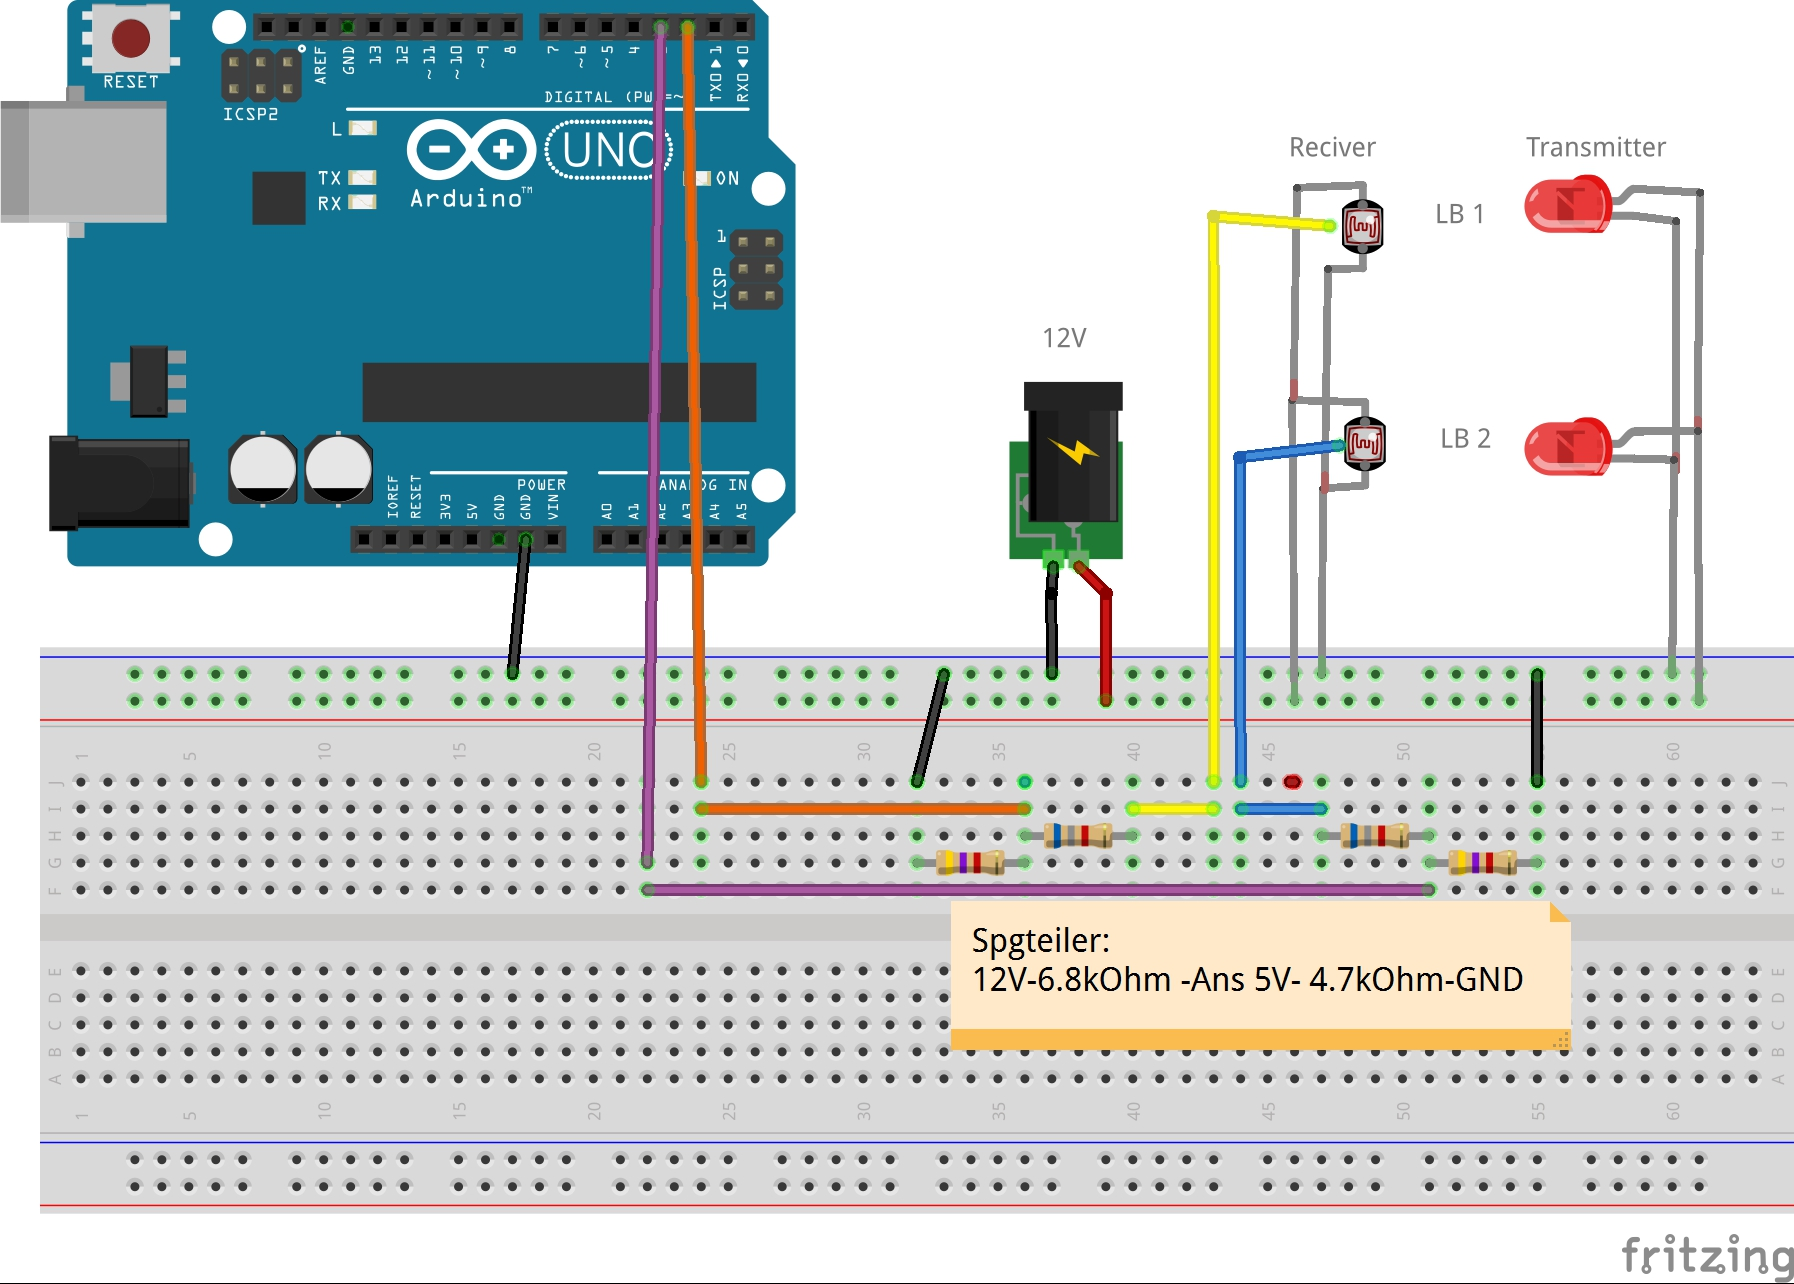
\includegraphics[width=\textwidth]{images/fritzing.jpg}
    \caption{Anschluss des Arduino Uno}
    \label{fig:ArdAns}
\end{figure}

